% mainfile: ../../../../master.tex
\subsection{Migration of nucleic acids in agarose gel}
% The part of the label after the colon must match the file name. Otherwise,
% conditional compilation based on task labels does NOT work.
\label{task:20180117_cj1}
\tags{lab,pcr,exp,emp}
\authors{cj}
%\files{}
%\persons{}


\subsubsection{1\% Agarose gel preparation}

\begin{enumerate}
\item measure with erlenmeyer 75~mL of 1\% agarose gel
\sidenote{The 1\% agarose gel is kept at 60\degree C in the gel room.}
\item warm up the erlenmeyer for 15s in microwave: agarose will be more fluid and it will avoid bubbles when casting the gel
\item add 3.75~\textmu L of SYBR Safe to the agarose while swirling \todo[noline, backgroundcolor=grass, bordercolor=white]{SYBR Safe by Invitrogen, 10,000X in \gls{dmso}}
\item cast the gel with the comb (for 20 wells)
\item let the gel set for 20 min
\end{enumerate}

\subsubsection{\gls{pcr} products preparation}

With a multichanel pipette:
\begin{itemize}
\item 5~\textmu L of each sample of PCR product
\item 5~\textmu L of blue dye (bromothymol blue)
\item tap gently tubes to mix up everything
\item centrifuge briefly to bring all the liquid to the bottom
\end{itemize}

\subsubsection{Electrophoresis}

For this electrophoresis migration, we run:
\begin{itemize}
\item 9~\textmu L of each sample of PCR product 
\item 5~\textmu L of the 1~kb ladder
\item 5~\textmu L of the 100~pb ladder
\end{itemize}

\begin{enumerate}
\item place the agarose gel into the gel box (electrophoresis unit) containing TAE buffer
\item load 5~\textmu L of molecular weight ladder into the first and last lane of the gel
\item load 9~\textmu L of each sample into the additional wells of the gel
\item run for 50~min with the \gls{eps} 301 at 100~V, 400~mA
\item visualize your \gls{dna} fragments with \gls{uv} lights
\end{enumerate}

\begin{figure}[H] % position of the figure 
    \centering
    \caption{Picture of 1\% agarose gel after 50 minute-long electrophoresis migration of \gls{pcr} products obtained with \gls{emp} primers, OneTaq\cR Hot Start DNA polymerase and from \gls{cdna} and \gls{dna} extrated from cultures.}
    \label{fig:20180117_OneTaq_EMP_cDNA2}
    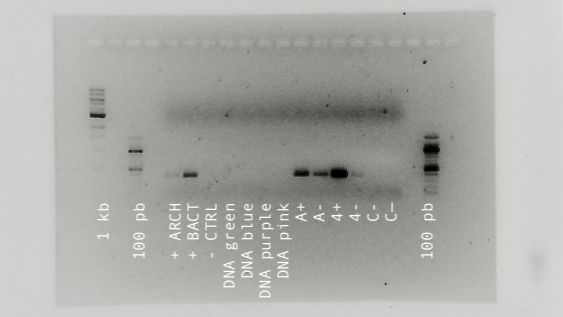
\includegraphics[width=\textwidth]{graphics/pic/20180117_OneTaq_EMP_cDNA2.png}
\end{figure}

Figure \ref{fig:20170810_PCR_EMP_OneStart_OSD_invert} shows results that are consistent with the Qubit\texttrademark~ dsDNA BR Assay. It confirms that I was able to retrieve RNA from bacterial cultures {\color{Lavender} \texttt{423 10M1}} and {\color{Rose} \texttt{ALMIX}}, and that I was able to reverse-transcribe the RNA in cDNA and eventually amplify the cDNA with bacterial primers. It is important to note that the negative control {\color{Aqua} \texttt{C-}} and {\color{Aqua} \texttt{C-~-}} of the extraction are negative, which confirms that there was no contamination during the extraction process. However, the negative control of the reverse transcription for {\color{Rose} \texttt{ALMIX}} labeled \texttt{A-} is not negative which reveals a contamination. This contamination might come from the reagents of the First Strand cDNA Synthesis Kit which is very old (and expired!). Regarding the DNA extracts, there is no amplification at all which was expected as the concentrations of DNA in these samples were below teh detetction levels, which confirms that there was very likely no DNA at all and that I was not able to extract the DNA from the cultured cells.
